% Options for packages loaded elsewhere
\PassOptionsToPackage{unicode}{hyperref}
\PassOptionsToPackage{hyphens}{url}
\PassOptionsToPackage{dvipsnames,svgnames,x11names}{xcolor}
%
\documentclass[
  letterpaper,
  DIV=11,
  numbers=noendperiod]{scrartcl}

\usepackage{amsmath,amssymb}
\usepackage{lmodern}
\usepackage{iftex}
\ifPDFTeX
  \usepackage[T1]{fontenc}
  \usepackage[utf8]{inputenc}
  \usepackage{textcomp} % provide euro and other symbols
\else % if luatex or xetex
  \usepackage{unicode-math}
  \defaultfontfeatures{Scale=MatchLowercase}
  \defaultfontfeatures[\rmfamily]{Ligatures=TeX,Scale=1}
\fi
% Use upquote if available, for straight quotes in verbatim environments
\IfFileExists{upquote.sty}{\usepackage{upquote}}{}
\IfFileExists{microtype.sty}{% use microtype if available
  \usepackage[]{microtype}
  \UseMicrotypeSet[protrusion]{basicmath} % disable protrusion for tt fonts
}{}
\makeatletter
\@ifundefined{KOMAClassName}{% if non-KOMA class
  \IfFileExists{parskip.sty}{%
    \usepackage{parskip}
  }{% else
    \setlength{\parindent}{0pt}
    \setlength{\parskip}{6pt plus 2pt minus 1pt}}
}{% if KOMA class
  \KOMAoptions{parskip=half}}
\makeatother
\usepackage{xcolor}
\setlength{\emergencystretch}{3em} % prevent overfull lines
\setcounter{secnumdepth}{-\maxdimen} % remove section numbering
% Make \paragraph and \subparagraph free-standing
\ifx\paragraph\undefined\else
  \let\oldparagraph\paragraph
  \renewcommand{\paragraph}[1]{\oldparagraph{#1}\mbox{}}
\fi
\ifx\subparagraph\undefined\else
  \let\oldsubparagraph\subparagraph
  \renewcommand{\subparagraph}[1]{\oldsubparagraph{#1}\mbox{}}
\fi

\usepackage{color}
\usepackage{fancyvrb}
\newcommand{\VerbBar}{|}
\newcommand{\VERB}{\Verb[commandchars=\\\{\}]}
\DefineVerbatimEnvironment{Highlighting}{Verbatim}{commandchars=\\\{\}}
% Add ',fontsize=\small' for more characters per line
\usepackage{framed}
\definecolor{shadecolor}{RGB}{241,243,245}
\newenvironment{Shaded}{\begin{snugshade}}{\end{snugshade}}
\newcommand{\AlertTok}[1]{\textcolor[rgb]{0.68,0.00,0.00}{#1}}
\newcommand{\AnnotationTok}[1]{\textcolor[rgb]{0.37,0.37,0.37}{#1}}
\newcommand{\AttributeTok}[1]{\textcolor[rgb]{0.40,0.45,0.13}{#1}}
\newcommand{\BaseNTok}[1]{\textcolor[rgb]{0.68,0.00,0.00}{#1}}
\newcommand{\BuiltInTok}[1]{\textcolor[rgb]{0.00,0.23,0.31}{#1}}
\newcommand{\CharTok}[1]{\textcolor[rgb]{0.13,0.47,0.30}{#1}}
\newcommand{\CommentTok}[1]{\textcolor[rgb]{0.37,0.37,0.37}{#1}}
\newcommand{\CommentVarTok}[1]{\textcolor[rgb]{0.37,0.37,0.37}{\textit{#1}}}
\newcommand{\ConstantTok}[1]{\textcolor[rgb]{0.56,0.35,0.01}{#1}}
\newcommand{\ControlFlowTok}[1]{\textcolor[rgb]{0.00,0.23,0.31}{#1}}
\newcommand{\DataTypeTok}[1]{\textcolor[rgb]{0.68,0.00,0.00}{#1}}
\newcommand{\DecValTok}[1]{\textcolor[rgb]{0.68,0.00,0.00}{#1}}
\newcommand{\DocumentationTok}[1]{\textcolor[rgb]{0.37,0.37,0.37}{\textit{#1}}}
\newcommand{\ErrorTok}[1]{\textcolor[rgb]{0.68,0.00,0.00}{#1}}
\newcommand{\ExtensionTok}[1]{\textcolor[rgb]{0.00,0.23,0.31}{#1}}
\newcommand{\FloatTok}[1]{\textcolor[rgb]{0.68,0.00,0.00}{#1}}
\newcommand{\FunctionTok}[1]{\textcolor[rgb]{0.28,0.35,0.67}{#1}}
\newcommand{\ImportTok}[1]{\textcolor[rgb]{0.00,0.46,0.62}{#1}}
\newcommand{\InformationTok}[1]{\textcolor[rgb]{0.37,0.37,0.37}{#1}}
\newcommand{\KeywordTok}[1]{\textcolor[rgb]{0.00,0.23,0.31}{#1}}
\newcommand{\NormalTok}[1]{\textcolor[rgb]{0.00,0.23,0.31}{#1}}
\newcommand{\OperatorTok}[1]{\textcolor[rgb]{0.37,0.37,0.37}{#1}}
\newcommand{\OtherTok}[1]{\textcolor[rgb]{0.00,0.23,0.31}{#1}}
\newcommand{\PreprocessorTok}[1]{\textcolor[rgb]{0.68,0.00,0.00}{#1}}
\newcommand{\RegionMarkerTok}[1]{\textcolor[rgb]{0.00,0.23,0.31}{#1}}
\newcommand{\SpecialCharTok}[1]{\textcolor[rgb]{0.37,0.37,0.37}{#1}}
\newcommand{\SpecialStringTok}[1]{\textcolor[rgb]{0.13,0.47,0.30}{#1}}
\newcommand{\StringTok}[1]{\textcolor[rgb]{0.13,0.47,0.30}{#1}}
\newcommand{\VariableTok}[1]{\textcolor[rgb]{0.07,0.07,0.07}{#1}}
\newcommand{\VerbatimStringTok}[1]{\textcolor[rgb]{0.13,0.47,0.30}{#1}}
\newcommand{\WarningTok}[1]{\textcolor[rgb]{0.37,0.37,0.37}{\textit{#1}}}

\providecommand{\tightlist}{%
  \setlength{\itemsep}{0pt}\setlength{\parskip}{0pt}}\usepackage{longtable,booktabs,array}
\usepackage{calc} % for calculating minipage widths
% Correct order of tables after \paragraph or \subparagraph
\usepackage{etoolbox}
\makeatletter
\patchcmd\longtable{\par}{\if@noskipsec\mbox{}\fi\par}{}{}
\makeatother
% Allow footnotes in longtable head/foot
\IfFileExists{footnotehyper.sty}{\usepackage{footnotehyper}}{\usepackage{footnote}}
\makesavenoteenv{longtable}
\usepackage{graphicx}
\makeatletter
\def\maxwidth{\ifdim\Gin@nat@width>\linewidth\linewidth\else\Gin@nat@width\fi}
\def\maxheight{\ifdim\Gin@nat@height>\textheight\textheight\else\Gin@nat@height\fi}
\makeatother
% Scale images if necessary, so that they will not overflow the page
% margins by default, and it is still possible to overwrite the defaults
% using explicit options in \includegraphics[width, height, ...]{}
\setkeys{Gin}{width=\maxwidth,height=\maxheight,keepaspectratio}
% Set default figure placement to htbp
\makeatletter
\def\fps@figure{htbp}
\makeatother

\KOMAoption{captions}{tableheading}
\makeatletter
\makeatother
\makeatletter
\makeatother
\makeatletter
\@ifpackageloaded{caption}{}{\usepackage{caption}}
\AtBeginDocument{%
\ifdefined\contentsname
  \renewcommand*\contentsname{Table of contents}
\else
  \newcommand\contentsname{Table of contents}
\fi
\ifdefined\listfigurename
  \renewcommand*\listfigurename{List of Figures}
\else
  \newcommand\listfigurename{List of Figures}
\fi
\ifdefined\listtablename
  \renewcommand*\listtablename{List of Tables}
\else
  \newcommand\listtablename{List of Tables}
\fi
\ifdefined\figurename
  \renewcommand*\figurename{Figure}
\else
  \newcommand\figurename{Figure}
\fi
\ifdefined\tablename
  \renewcommand*\tablename{Table}
\else
  \newcommand\tablename{Table}
\fi
}
\@ifpackageloaded{float}{}{\usepackage{float}}
\floatstyle{ruled}
\@ifundefined{c@chapter}{\newfloat{codelisting}{h}{lop}}{\newfloat{codelisting}{h}{lop}[chapter]}
\floatname{codelisting}{Listing}
\newcommand*\listoflistings{\listof{codelisting}{List of Listings}}
\makeatother
\makeatletter
\@ifpackageloaded{caption}{}{\usepackage{caption}}
\@ifpackageloaded{subcaption}{}{\usepackage{subcaption}}
\makeatother
\makeatletter
\@ifpackageloaded{tcolorbox}{}{\usepackage[many]{tcolorbox}}
\makeatother
\makeatletter
\@ifundefined{shadecolor}{\definecolor{shadecolor}{rgb}{.97, .97, .97}}
\makeatother
\makeatletter
\makeatother
\ifLuaTeX
  \usepackage{selnolig}  % disable illegal ligatures
\fi
\IfFileExists{bookmark.sty}{\usepackage{bookmark}}{\usepackage{hyperref}}
\IfFileExists{xurl.sty}{\usepackage{xurl}}{} % add URL line breaks if available
\urlstyle{same} % disable monospaced font for URLs
\hypersetup{
  pdftitle={Robby - Homework 1},
  colorlinks=true,
  linkcolor={blue},
  filecolor={Maroon},
  citecolor={Blue},
  urlcolor={Blue},
  pdfcreator={LaTeX via pandoc}}

\title{Robby - Homework 1}
\author{}
\date{}

\begin{document}
\maketitle
\ifdefined\Shaded\renewenvironment{Shaded}{\begin{tcolorbox}[enhanced, frame hidden, borderline west={3pt}{0pt}{shadecolor}, boxrule=0pt, interior hidden, breakable, sharp corners]}{\end{tcolorbox}}\fi

\hypertarget{quarto}{%
\subsection{Quarto}\label{quarto}}

Quarto enables you to weave together content and executable code into a
finished document. To learn more about Quarto see
\url{https://quarto.org}.

\hypertarget{running-code}{%
\subsection{Running Code}\label{running-code}}

When you click the \textbf{Render} button a document will be generated
that includes both content and the output of embedded code. You can
embed code like this:

\begin{Shaded}
\begin{Highlighting}[]
\DecValTok{1} \SpecialCharTok{+} \DecValTok{1}
\end{Highlighting}
\end{Shaded}

\begin{verbatim}
[1] 2
\end{verbatim}

You can add options to executable code like this

\begin{Shaded}
\begin{Highlighting}[]
\CommentTok{\#|echo: false}
\DecValTok{2} \SpecialCharTok{*} \DecValTok{2}
\end{Highlighting}
\end{Shaded}

\begin{verbatim}
[1] 4
\end{verbatim}

The \texttt{echo:\ false} option disables the printing of code (only
output is displayed).

\hypertarget{point-process-homework-basics}{%
\section{Point Process Homework
(Basics)}\label{point-process-homework-basics}}

\hypertarget{problem-1}{%
\subsection{Problem 1}\label{problem-1}}

What are the two components needed to define a spatial point process?

\begin{quote}
\begin{enumerate}
\def\labelenumi{\arabic{enumi}.}
\tightlist
\item
  Event Locations (where and event did occur)
\item
  Event Space (where an event could occur)
\end{enumerate}
\end{quote}

\hypertarget{problem-2}{%
\subsection{Problem 2}\label{problem-2}}

What are the main components that define a homogeneous Poisson point
process?

\begin{quote}
\begin{enumerate}
\def\labelenumi{\arabic{enumi}.}
\tightlist
\item
  Stationarity and a constant intensity parameter Lambda
\item
  Complete Spatial Randomness (events are uniformly distributed over the
  study region)
\end{enumerate}
\end{quote}

\hypertarget{problem-3}{%
\subsection{Problem 3}\label{problem-3}}

What is the main difference between a homogeneous and heterogeneous
point process (pp)?

\begin{quote}
The main difference between the two point processes is that the
intensity of events within the study region is constant for the
homogeneous pp and not constant for the heterogeneous pp.
\end{quote}

\hypertarget{problem-4}{%
\subsection{Problem 4}\label{problem-4}}

Describe the differences between a regular, clustered, and homogeneous
(CSR) Poisson pp?

\begin{quote}
One can think of the relationship (and the difference between these
point patterns) as a spectrum ranging from a regular distribution of
points wherein no clustering is observed, moving to CSR in which each
event location is uniformly distributed and independent of each other
event location, and finally on the other end of the spectrum is
clustering, in which event locations are grouped up more than would be
random.
\end{quote}

\hypertarget{problem-5}{%
\subsection{Problem 5}\label{problem-5}}

For this problem, I was able to create a plot for each realization using
code from Dr.~French's github repo.

\hypertarget{regular-point-process}{%
\subsubsection{Regular Point Process}\label{regular-point-process}}

\begin{Shaded}
\begin{Highlighting}[]
\FunctionTok{library}\NormalTok{(splancs)}
\end{Highlighting}
\end{Shaded}

\begin{verbatim}
Warning: package 'splancs' was built under R version 4.2.3
\end{verbatim}

\begin{verbatim}
Loading required package: sp
\end{verbatim}

\begin{verbatim}
Warning: package 'sp' was built under R version 4.2.3
\end{verbatim}

\begin{verbatim}
The legacy packages maptools, rgdal, and rgeos, underpinning the sp package,
which was just loaded, will retire in October 2023.
Please refer to R-spatial evolution reports for details, especially
https://r-spatial.org/r/2023/05/15/evolution4.html.
It may be desirable to make the sf package available;
package maintainers should consider adding sf to Suggests:.
The sp package is now running under evolution status 2
     (status 2 uses the sf package in place of rgdal)
\end{verbatim}

\begin{verbatim}

Spatial Point Pattern Analysis Code in S-Plus
 
 Version 2 - Spatial and Space-Time analysis
\end{verbatim}

\begin{Shaded}
\begin{Highlighting}[]
\FunctionTok{library}\NormalTok{(spatial)}

\CommentTok{\# Regular PP Set Up}
\FunctionTok{set.seed}\NormalTok{(}\DecValTok{1}\NormalTok{) }\CommentTok{\# for reproducability}
\FunctionTok{ppregion}\NormalTok{(}\AttributeTok{xl =} \DecValTok{0}\NormalTok{, }\AttributeTok{xu =} \DecValTok{1}\NormalTok{, }\AttributeTok{yl =} \DecValTok{0}\NormalTok{, }\AttributeTok{yu =} \DecValTok{1}\NormalTok{)}

\CommentTok{\# Simulate 30 events from a Strauss process with probability c of other events}
\CommentTok{\# within distance r of other events.}
\NormalTok{test }\OtherTok{\textless{}{-}} \FunctionTok{Strauss}\NormalTok{(}\DecValTok{30}\NormalTok{, }\AttributeTok{c =} \DecValTok{0}\NormalTok{, }\AttributeTok{r =} \FloatTok{0.05}\NormalTok{)}
\FunctionTok{plot}\NormalTok{(test, }\AttributeTok{xlim =} \DecValTok{0}\SpecialCharTok{:}\DecValTok{1}\NormalTok{, }\AttributeTok{ylim =} \DecValTok{0}\SpecialCharTok{:}\DecValTok{1}\NormalTok{, }\AttributeTok{xlab =} \StringTok{"u"}\NormalTok{, }\AttributeTok{ylab =} \StringTok{"v"}\NormalTok{, }\AttributeTok{cex.lab =} \FloatTok{1.5}\NormalTok{, }\AttributeTok{cex.axis =} \FloatTok{1.1}\NormalTok{)}
\FunctionTok{title}\NormalTok{(}\StringTok{"Regular"}\NormalTok{)}
\end{Highlighting}
\end{Shaded}

\begin{figure}[H]

{\centering 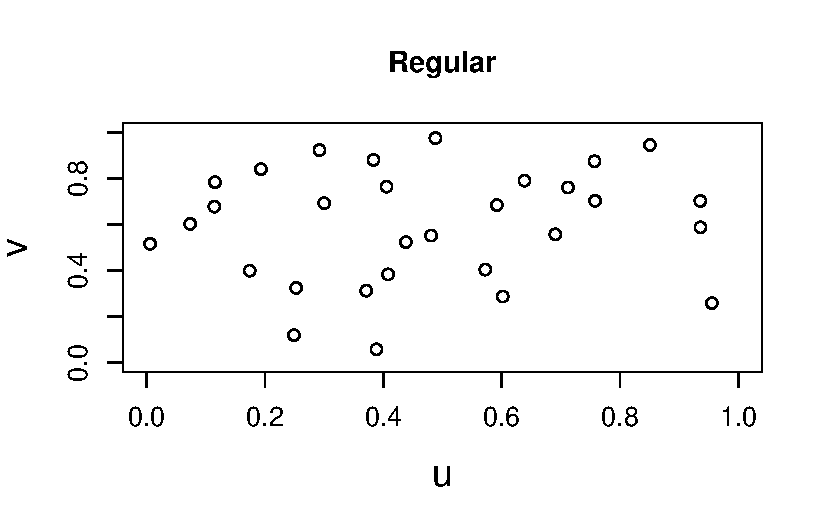
\includegraphics{robby_homework_1_files/figure-pdf/unnamed-chunk-3-1.pdf}

}

\end{figure}

\hypertarget{clustered-point-process}{%
\subsubsection{Clustered Point Process}\label{clustered-point-process}}

\begin{Shaded}
\begin{Highlighting}[]
\CommentTok{\# domain is unit square}
\NormalTok{domain }\OtherTok{=} \FunctionTok{cbind}\NormalTok{(}\FunctionTok{c}\NormalTok{(}\DecValTok{0}\NormalTok{,}\DecValTok{0}\NormalTok{,}\DecValTok{1}\NormalTok{,}\DecValTok{1}\NormalTok{), }\FunctionTok{c}\NormalTok{(}\DecValTok{0}\NormalTok{,}\DecValTok{1}\NormalTok{,}\DecValTok{1}\NormalTok{,}\DecValTok{0}\NormalTok{))}


\NormalTok{test }\OtherTok{\textless{}{-}} \FunctionTok{pcp.sim}\NormalTok{(}\AttributeTok{rho =} \DecValTok{5}\NormalTok{, }\AttributeTok{m =} \DecValTok{15}\NormalTok{, }\AttributeTok{s2 =} \FloatTok{0.01}\NormalTok{, }\AttributeTok{region.poly =}\NormalTok{ domain)}
\FunctionTok{plot}\NormalTok{(test, }\AttributeTok{xlim =} \DecValTok{0}\SpecialCharTok{:}\DecValTok{1}\NormalTok{, }\AttributeTok{ylim =} \DecValTok{0}\SpecialCharTok{:}\DecValTok{1}\NormalTok{, }\AttributeTok{xlab =} \StringTok{"u"}\NormalTok{, }\AttributeTok{ylab =} \StringTok{"v"}\NormalTok{, }
     \AttributeTok{cex.lab =} \FloatTok{1.5}\NormalTok{, }\AttributeTok{cex.axis =} \FloatTok{1.1}\NormalTok{)}
\FunctionTok{title}\NormalTok{(}\StringTok{"Clustered"}\NormalTok{)}
\end{Highlighting}
\end{Shaded}

\begin{figure}[H]

{\centering 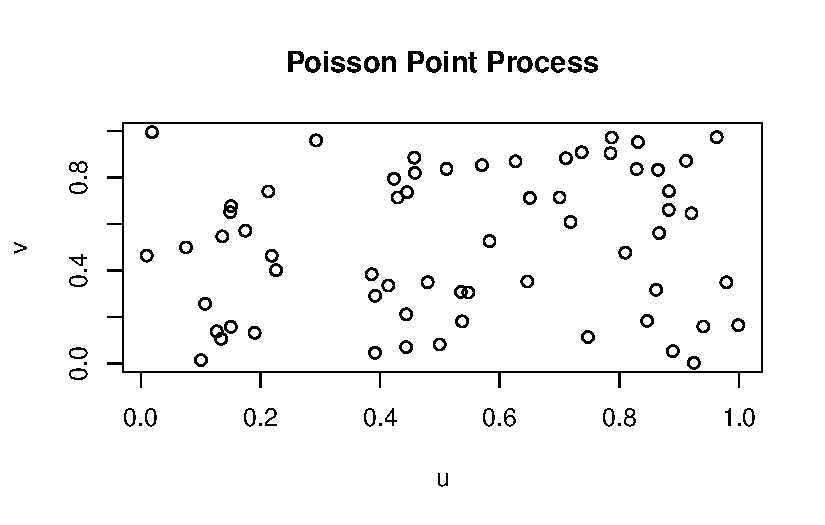
\includegraphics{robby_homework_1_files/figure-pdf/unnamed-chunk-4-1.pdf}

}

\end{figure}

\hypertarget{csr-poisson-point-process}{%
\subsubsection{CSR Poisson Point
Process}\label{csr-poisson-point-process}}

\begin{Shaded}
\begin{Highlighting}[]
\FunctionTok{library}\NormalTok{(spatstat)}
\end{Highlighting}
\end{Shaded}

\begin{verbatim}
Warning: package 'spatstat' was built under R version 4.2.3
\end{verbatim}

\begin{verbatim}
Loading required package: spatstat.data
\end{verbatim}

\begin{verbatim}
Warning: package 'spatstat.data' was built under R version 4.2.3
\end{verbatim}

\begin{verbatim}
Loading required package: spatstat.geom
\end{verbatim}

\begin{verbatim}
Warning: package 'spatstat.geom' was built under R version 4.2.3
\end{verbatim}

\begin{verbatim}
spatstat.geom 3.2-4
\end{verbatim}

\begin{verbatim}
Loading required package: spatstat.random
\end{verbatim}

\begin{verbatim}
Warning: package 'spatstat.random' was built under R version 4.2.3
\end{verbatim}

\begin{verbatim}
spatstat.random 3.1-5
\end{verbatim}

\begin{verbatim}
Loading required package: spatstat.explore
\end{verbatim}

\begin{verbatim}
Warning: package 'spatstat.explore' was built under R version 4.2.3
\end{verbatim}

\begin{verbatim}
Loading required package: nlme
\end{verbatim}

\begin{verbatim}
spatstat.explore 3.2-1
\end{verbatim}

\begin{verbatim}
Loading required package: spatstat.model
\end{verbatim}

\begin{verbatim}
Warning: package 'spatstat.model' was built under R version 4.2.3
\end{verbatim}

\begin{verbatim}
Loading required package: rpart
\end{verbatim}

\begin{verbatim}
spatstat.model 3.2-4
\end{verbatim}

\begin{verbatim}

Attaching package: 'spatstat.model'
\end{verbatim}

\begin{verbatim}
The following object is masked from 'package:spatial':

    Strauss
\end{verbatim}

\begin{verbatim}
Loading required package: spatstat.linnet
\end{verbatim}

\begin{verbatim}
Warning: package 'spatstat.linnet' was built under R version 4.2.3
\end{verbatim}

\begin{verbatim}
spatstat.linnet 3.1-1
\end{verbatim}

\begin{verbatim}

spatstat 3.0-6 
For an introduction to spatstat, type 'beginner' 
\end{verbatim}

\begin{Shaded}
\begin{Highlighting}[]
\NormalTok{poi }\OtherTok{\textless{}{-}} \FunctionTok{rpoispp}\NormalTok{(}\DecValTok{50}\NormalTok{)}
\FunctionTok{plot}\NormalTok{(poi,}\AttributeTok{xlim =} \DecValTok{0}\SpecialCharTok{:}\DecValTok{1}\NormalTok{, }\AttributeTok{ylim =} \DecValTok{0}\SpecialCharTok{:}\DecValTok{1}\NormalTok{, }\AttributeTok{xlab =} \StringTok{"u"}\NormalTok{, }\AttributeTok{ylab =} \StringTok{"v"}\NormalTok{, }
     \AttributeTok{cex.lab =} \FloatTok{1.5}\NormalTok{, }\AttributeTok{cex.axis =} \FloatTok{1.1}\NormalTok{)}
\FunctionTok{title}\NormalTok{(}\StringTok{"CSR Poisson Point Process"}\NormalTok{)}
\end{Highlighting}
\end{Shaded}

\begin{figure}[H]

{\centering 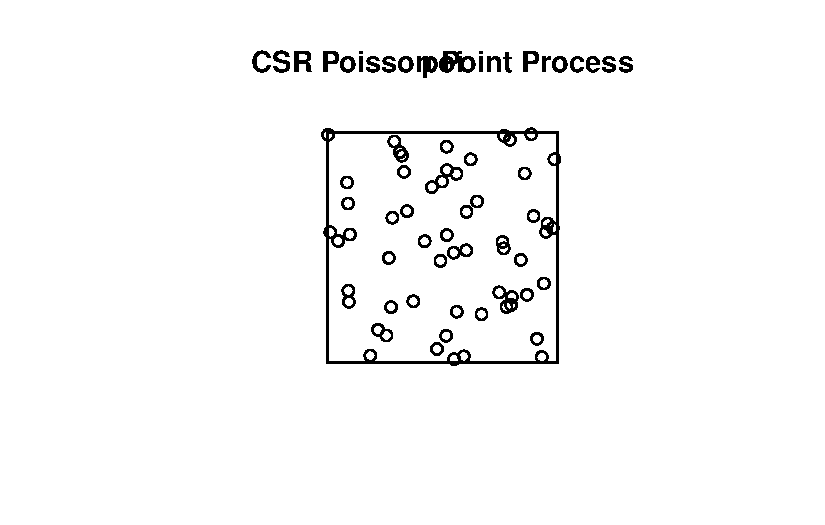
\includegraphics{robby_homework_1_files/figure-pdf/unnamed-chunk-5-1.pdf}

}

\end{figure}

\hypertarget{problem-6}{%
\subsection{Problem 6}\label{problem-6}}

\begin{Shaded}
\begin{Highlighting}[]
\FunctionTok{library}\NormalTok{(spatstat)}
\NormalTok{h1 }\OtherTok{\textless{}{-}} \FunctionTok{rpoispp}\NormalTok{(}\DecValTok{50}\NormalTok{)}
\FunctionTok{plot}\NormalTok{(h1)}
\end{Highlighting}
\end{Shaded}

\begin{figure}[H]

{\centering 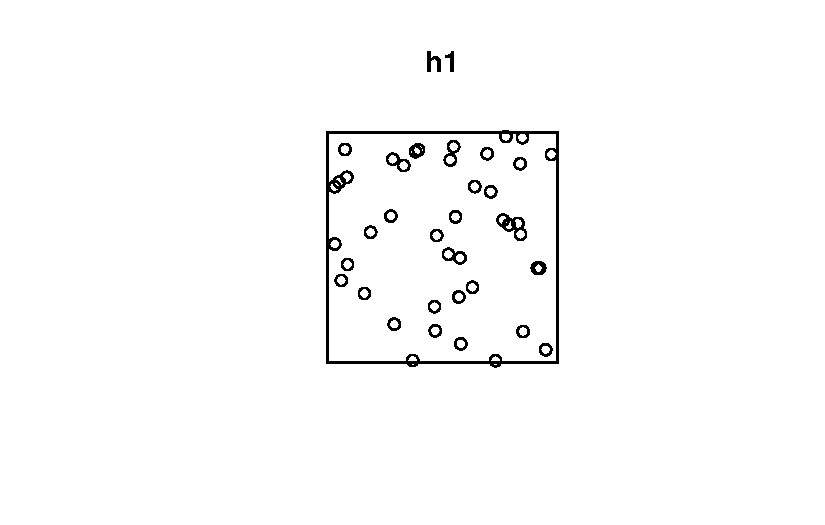
\includegraphics{robby_homework_1_files/figure-pdf/unnamed-chunk-6-1.pdf}

}

\end{figure}

\begin{quote}
The h1 plot shows a seemingly random realization of 50 points. While
there is little evidence of overlapping event locations, we can see at
least one such pair of events which means this is not a regular plot,
and not indicative of clustering. Therefore, it seems the h1 plot could
be bompatible with CSR.
\end{quote}

\hypertarget{problem-7}{%
\subsection{Problem 7}\label{problem-7}}

\begin{Shaded}
\begin{Highlighting}[]
\NormalTok{rcsr }\OtherTok{\textless{}{-}} \ControlFlowTok{function}\NormalTok{(lambda)\{}
\NormalTok{  region }\OtherTok{=} \FunctionTok{cbind}\NormalTok{(}\FunctionTok{c}\NormalTok{(}\DecValTok{1}\NormalTok{,}\DecValTok{0}\NormalTok{,}\DecValTok{0}\NormalTok{,}\DecValTok{1}\NormalTok{), }\FunctionTok{c}\NormalTok{(}\DecValTok{1}\NormalTok{,}\DecValTok{1}\NormalTok{,}\DecValTok{0}\NormalTok{,}\DecValTok{0}\NormalTok{))}
\NormalTok{  N }\OtherTok{=}\NormalTok{ lambda}
\NormalTok{  points }\OtherTok{=} \FunctionTok{csr}\NormalTok{(region,N)}
\NormalTok{  wreg }\OtherTok{=} \FunctionTok{owin}\NormalTok{(}\AttributeTok{poly =}\NormalTok{ region)}
\NormalTok{  pp\_1 }\OtherTok{=} \FunctionTok{ppp}\NormalTok{(}\AttributeTok{x=}\NormalTok{points[,}\DecValTok{1}\NormalTok{],}\AttributeTok{y=}\NormalTok{points[,}\DecValTok{2}\NormalTok{],}\AttributeTok{window =}\NormalTok{ wreg)}
  \FunctionTok{return}\NormalTok{(pp\_1)}
\NormalTok{\}}
\end{Highlighting}
\end{Shaded}

\begin{Shaded}
\begin{Highlighting}[]
\NormalTok{lambda }\OtherTok{=} \DecValTok{50}
\NormalTok{h2 }\OtherTok{\textless{}{-}} \FunctionTok{rcsr}\NormalTok{(lambda)}
\FunctionTok{plot}\NormalTok{(h2)}
\end{Highlighting}
\end{Shaded}

\begin{figure}[H]

{\centering 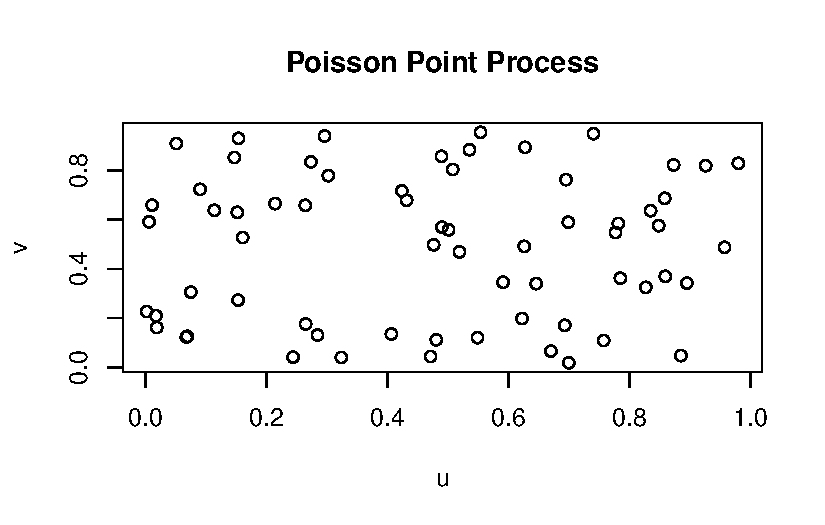
\includegraphics{robby_homework_1_files/figure-pdf/unnamed-chunk-8-1.pdf}

}

\end{figure}

\hypertarget{problem-8}{%
\subsection{Problem 8}\label{problem-8}}

\begin{quote}
\begin{enumerate}
\def\labelenumi{\arabic{enumi}.}
\tightlist
\item
  Draw a single data set from the rpoispp function. Use the density
  function to estimate the intensity function for the simulated data
  set. Compute the difference between the maximum and minimum estimated
  intensity values.
\end{enumerate}
\end{quote}

\begin{Shaded}
\begin{Highlighting}[]
\NormalTok{dim }\OtherTok{=} \DecValTok{2}
\NormalTok{df }\OtherTok{=} \FunctionTok{rpoispp}\NormalTok{(}\DecValTok{50}\NormalTok{)}
\NormalTok{bx }\OtherTok{=} \FunctionTok{sd}\NormalTok{(df}\SpecialCharTok{$}\NormalTok{x)}\SpecialCharTok{*}\FunctionTok{length}\NormalTok{(df}\SpecialCharTok{$}\NormalTok{x)}\SpecialCharTok{\^{}}\NormalTok{(}\SpecialCharTok{{-}}\DecValTok{1}\SpecialCharTok{/}\NormalTok{(dim}\SpecialCharTok{+}\DecValTok{4}\NormalTok{))}
\NormalTok{by }\OtherTok{=} \FunctionTok{sd}\NormalTok{(df}\SpecialCharTok{$}\NormalTok{y)}\SpecialCharTok{*}\FunctionTok{length}\NormalTok{(df}\SpecialCharTok{$}\NormalTok{y)}\SpecialCharTok{\^{}}\NormalTok{(}\SpecialCharTok{{-}}\DecValTok{1}\SpecialCharTok{/}\NormalTok{(dim}\SpecialCharTok{+}\DecValTok{4}\NormalTok{))}

\NormalTok{ix }\OtherTok{=} \FunctionTok{density}\NormalTok{(df,}\AttributeTok{sigma =} \FunctionTok{c}\NormalTok{(bx,by))}

\NormalTok{ix\_min }\OtherTok{=} \FunctionTok{min}\NormalTok{(ix}\SpecialCharTok{$}\NormalTok{v)}
\NormalTok{ix\_max }\OtherTok{=} \FunctionTok{max}\NormalTok{(ix}\SpecialCharTok{$}\NormalTok{v)}
\NormalTok{ix\_diff }\OtherTok{=}\NormalTok{ ix\_max }\SpecialCharTok{{-}}\NormalTok{ ix\_min}
\FunctionTok{print}\NormalTok{(ix\_diff)}
\end{Highlighting}
\end{Shaded}

\begin{verbatim}
[1] 63.93511
\end{verbatim}

\begin{quote}
\begin{enumerate}
\def\labelenumi{\arabic{enumi}.}
\setcounter{enumi}{1}
\tightlist
\item
  Draw a simulated data set from the `rcsr' function assuming lambda =
  50. Use the density function to estimate the intensity function of the
  simulated data set, and compute the diff between max and min intensity
  values.
\end{enumerate}
\end{quote}

\begin{Shaded}
\begin{Highlighting}[]
\NormalTok{dim }\OtherTok{=} \DecValTok{2}
\NormalTok{lambda }\OtherTok{=} \DecValTok{50}
\NormalTok{df }\OtherTok{=} \FunctionTok{rcsr}\NormalTok{(}\DecValTok{50}\NormalTok{)}
\NormalTok{bx }\OtherTok{=} \FunctionTok{sd}\NormalTok{(df}\SpecialCharTok{$}\NormalTok{x)}\SpecialCharTok{*}\FunctionTok{length}\NormalTok{(df}\SpecialCharTok{$}\NormalTok{x)}\SpecialCharTok{\^{}}\NormalTok{(}\SpecialCharTok{{-}}\DecValTok{1}\SpecialCharTok{/}\NormalTok{(dim}\SpecialCharTok{+}\DecValTok{4}\NormalTok{))}
\NormalTok{by }\OtherTok{=} \FunctionTok{sd}\NormalTok{(df}\SpecialCharTok{$}\NormalTok{y)}\SpecialCharTok{*}\FunctionTok{length}\NormalTok{(df}\SpecialCharTok{$}\NormalTok{y)}\SpecialCharTok{\^{}}\NormalTok{(}\SpecialCharTok{{-}}\DecValTok{1}\SpecialCharTok{/}\NormalTok{(dim}\SpecialCharTok{+}\DecValTok{4}\NormalTok{))}

\NormalTok{ix }\OtherTok{=} \FunctionTok{density}\NormalTok{(df,}\AttributeTok{sigma =} \FunctionTok{c}\NormalTok{(bx,by))}

\NormalTok{ix\_min }\OtherTok{=} \FunctionTok{min}\NormalTok{(ix}\SpecialCharTok{$}\NormalTok{v)}
\NormalTok{ix\_max }\OtherTok{=} \FunctionTok{max}\NormalTok{(ix}\SpecialCharTok{$}\NormalTok{v)}
\NormalTok{ix\_diff }\OtherTok{=}\NormalTok{ ix\_max }\SpecialCharTok{{-}}\NormalTok{ ix\_min}
\FunctionTok{print}\NormalTok{(ix\_diff)}
\end{Highlighting}
\end{Shaded}

\begin{verbatim}
[1] 40.67527
\end{verbatim}

\begin{quote}
\begin{enumerate}
\def\labelenumi{\arabic{enumi}.}
\setcounter{enumi}{2}
\tightlist
\item
  Repeat previous test 999 times
\end{enumerate}
\end{quote}

\begin{Shaded}
\begin{Highlighting}[]
\NormalTok{dim }\OtherTok{=} \DecValTok{2}
\NormalTok{lambda }\OtherTok{=} \DecValTok{50}
\NormalTok{result }\OtherTok{=} \FunctionTok{data.frame}\NormalTok{()}
\ControlFlowTok{for}\NormalTok{ (i }\ControlFlowTok{in} \DecValTok{1}\SpecialCharTok{:}\DecValTok{999}\NormalTok{) \{}
\NormalTok{  df }\OtherTok{=} \FunctionTok{rcsr}\NormalTok{(}\DecValTok{50}\NormalTok{)}
\NormalTok{  bx }\OtherTok{=} \FunctionTok{sd}\NormalTok{(df}\SpecialCharTok{$}\NormalTok{x)}\SpecialCharTok{*}\FunctionTok{length}\NormalTok{(df}\SpecialCharTok{$}\NormalTok{x)}\SpecialCharTok{\^{}}\NormalTok{(}\SpecialCharTok{{-}}\DecValTok{1}\SpecialCharTok{/}\NormalTok{(dim}\SpecialCharTok{+}\DecValTok{4}\NormalTok{))}
\NormalTok{  by }\OtherTok{=} \FunctionTok{sd}\NormalTok{(df}\SpecialCharTok{$}\NormalTok{y)}\SpecialCharTok{*}\FunctionTok{length}\NormalTok{(df}\SpecialCharTok{$}\NormalTok{y)}\SpecialCharTok{\^{}}\NormalTok{(}\SpecialCharTok{{-}}\DecValTok{1}\SpecialCharTok{/}\NormalTok{(dim}\SpecialCharTok{+}\DecValTok{4}\NormalTok{))}
  
\NormalTok{  ix }\OtherTok{=} \FunctionTok{density}\NormalTok{(df,}\AttributeTok{sigma =} \FunctionTok{c}\NormalTok{(bx,by))}
  
\NormalTok{  ix\_min }\OtherTok{=} \FunctionTok{min}\NormalTok{(ix}\SpecialCharTok{$}\NormalTok{v)}
\NormalTok{  ix\_max }\OtherTok{=} \FunctionTok{max}\NormalTok{(ix}\SpecialCharTok{$}\NormalTok{v)}
\NormalTok{  ix\_mean }\OtherTok{=} \FunctionTok{mean}\NormalTok{(ix}\SpecialCharTok{$}\NormalTok{v)}
\NormalTok{  ix\_diff }\OtherTok{=}\NormalTok{ ix\_max }\SpecialCharTok{{-}}\NormalTok{ ix\_min}
\NormalTok{  result[i,}\DecValTok{1}\NormalTok{] }\OtherTok{=}\NormalTok{ ix\_mean}
\NormalTok{\}}

\FunctionTok{print}\NormalTok{(result)}
\end{Highlighting}
\end{Shaded}

\begin{verbatim}
          V1
1   51.20840
2   50.50872
3   48.98157
4   51.23246
5   48.54668
6   49.19084
7   49.00356
8   49.93600
9   51.01645
10  49.34572
11  50.72501
12  50.01272
13  50.45802
14  48.71708
15  50.05886
16  49.61864
17  49.80207
18  49.81927
19  48.77529
20  50.59438
21  50.86967
22  51.00210
23  50.13837
24  49.07787
25  50.23642
26  49.44350
27  49.68044
28  48.00032
29  50.28944
30  50.72878
31  50.44209
32  49.03494
33  50.48470
34  47.62499
35  50.91520
36  49.37827
37  50.48519
38  50.55062
39  50.70995
40  50.48595
41  50.07753
42  49.99746
43  49.27817
44  49.45085
45  48.92574
46  47.90261
47  49.72455
48  51.18615
49  50.04381
50  50.31813
51  50.09108
52  50.82942
53  49.47500
54  50.20543
55  50.09682
56  49.35650
57  50.28836
58  50.27639
59  48.06579
60  51.00503
61  50.24824
62  49.04913
63  48.83715
64  48.99222
65  49.98587
66  50.19253
67  50.60761
68  49.25701
69  50.46134
70  49.08183
71  50.65696
72  50.28888
73  50.49669
74  50.53841
75  50.49712
76  50.58642
77  51.21353
78  51.04312
79  49.87619
80  48.59265
81  49.04887
82  49.42045
83  51.04180
84  48.53542
85  50.57396
86  48.91173
87  48.54118
88  48.08449
89  50.22193
90  50.68266
91  48.67077
92  51.30127
93  48.77500
94  51.27092
95  51.10563
96  49.56128
97  48.25444
98  49.22141
99  49.44251
100 49.24908
101 49.20574
102 49.99511
103 50.62923
104 49.97340
105 50.53333
106 49.09127
107 48.13468
108 50.68966
109 51.62401
110 50.37891
111 50.27952
112 49.16275
113 50.13214
114 50.81116
115 49.31838
116 49.75355
117 48.70517
118 50.75942
119 50.63227
120 50.51275
121 49.12151
122 49.87342
123 50.27107
124 49.14977
125 50.60568
126 50.95022
127 49.70862
128 49.69299
129 48.75983
130 50.33806
131 50.45458
132 49.89526
133 51.61954
134 52.62214
135 49.33616
136 51.20455
137 50.06568
138 50.79842
139 50.42331
140 49.95865
141 50.18689
142 49.44098
143 49.87315
144 49.74710
145 50.61834
146 50.02729
147 48.96852
148 49.69810
149 49.02671
150 50.36462
151 51.08340
152 50.43276
153 48.68925
154 48.36957
155 48.54139
156 49.74595
157 50.88119
158 49.39035
159 49.74920
160 50.81162
161 50.63196
162 47.31414
163 49.55819
164 49.73265
165 49.54027
166 48.22044
167 50.74793
168 49.01299
169 49.40838
170 49.10463
171 47.76389
172 50.51527
173 50.06402
174 49.39018
175 51.54460
176 48.77270
177 52.06513
178 50.63855
179 51.70733
180 47.98814
181 50.07133
182 49.24622
183 50.09171
184 50.06512
185 51.95921
186 48.71388
187 49.66682
188 51.30353
189 48.63961
190 51.30960
191 50.23530
192 49.51575
193 50.41169
194 50.26342
195 50.82632
196 50.88083
197 50.81387
198 49.93516
199 49.62669
200 49.70361
201 50.41636
202 51.28562
203 49.98241
204 51.92172
205 50.69117
206 48.23238
207 49.94715
208 50.95404
209 50.61679
210 49.63007
211 50.67833
212 50.32570
213 49.73546
214 50.82235
215 50.05397
216 49.74870
217 48.62164
218 49.30864
219 50.52383
220 50.56651
221 49.41158
222 50.03895
223 49.58045
224 50.40350
225 50.13220
226 50.55493
227 50.98432
228 48.92914
229 50.77042
230 51.16776
231 51.44339
232 51.45206
233 48.31868
234 49.46558
235 50.61208
236 50.15510
237 49.22088
238 50.11050
239 50.01040
240 49.78040
241 51.31311
242 50.03192
243 49.92216
244 48.10768
245 50.49213
246 49.04140
247 49.57491
248 47.66804
249 50.16818
250 49.55552
251 49.94489
252 50.66441
253 49.56813
254 49.08711
255 50.12144
256 49.22977
257 50.30746
258 50.56768
259 50.14956
260 49.33757
261 49.63987
262 49.80540
263 50.38737
264 51.53477
265 50.50781
266 49.27721
267 50.56201
268 49.56713
269 50.75554
270 48.49621
271 50.42312
272 50.16404
273 50.72390
274 50.62644
275 49.50456
276 50.39715
277 49.71195
278 48.45971
279 48.61443
280 50.31359
281 51.20969
282 51.14245
283 49.59128
284 48.96492
285 49.91721
286 49.35904
287 50.59663
288 47.66227
289 50.14021
290 50.32521
291 51.40468
292 49.87900
293 50.76687
294 50.99987
295 50.73324
296 49.15734
297 50.93268
298 51.06645
299 50.32826
300 48.85163
301 51.02134
302 48.36434
303 48.89884
304 49.65181
305 50.87820
306 51.72391
307 50.76652
308 51.73278
309 50.34804
310 52.20532
311 51.14913
312 49.92017
313 50.72727
314 50.82612
315 49.42290
316 49.40913
317 49.85423
318 48.19041
319 51.51440
320 50.72936
321 49.98754
322 50.10738
323 49.77344
324 50.69906
325 49.53744
326 50.56480
327 50.01754
328 50.61664
329 49.62849
330 47.01418
331 49.36794
332 49.92263
333 50.45362
334 49.49777
335 51.52525
336 49.49306
337 49.37968
338 50.96766
339 50.04882
340 49.45315
341 49.53293
342 49.70617
343 48.77802
344 48.97690
345 50.35965
346 49.40281
347 50.04302
348 49.78107
349 50.51648
350 48.28708
351 48.32304
352 50.25348
353 49.05279
354 49.29982
355 49.71261
356 51.88856
357 49.16070
358 51.03777
359 50.36454
360 49.59618
361 50.52962
362 49.70980
363 50.61746
364 50.94676
365 51.34811
366 49.52922
367 48.19053
368 49.81367
369 50.06908
370 49.17718
371 49.31179
372 50.78159
373 49.62732
374 50.13522
375 50.62441
376 49.92736
377 50.43852
378 49.95909
379 49.04495
380 49.71334
381 49.65681
382 49.60562
383 49.31252
384 50.38098
385 50.16889
386 49.95911
387 49.58820
388 50.72856
389 48.09556
390 49.36231
391 50.16907
392 49.93177
393 47.70528
394 49.14011
395 48.35755
396 48.31220
397 51.03712
398 49.60103
399 49.07193
400 49.76234
401 49.64588
402 50.63047
403 49.59091
404 50.56699
405 50.24411
406 50.38168
407 50.22426
408 49.92379
409 49.17435
410 49.69730
411 48.17751
412 50.12088
413 49.23941
414 49.58302
415 50.28417
416 50.32845
417 50.53969
418 50.49449
419 51.03792
420 49.73907
421 50.89648
422 50.98911
423 49.65821
424 50.10121
425 49.60629
426 51.70395
427 48.29235
428 50.47566
429 49.50062
430 50.05751
431 47.59016
432 50.98409
433 49.14746
434 50.92184
435 52.27301
436 50.59860
437 47.90414
438 50.63346
439 50.04113
440 49.75552
441 47.72856
442 50.18756
443 50.35499
444 48.18456
445 49.07183
446 48.77239
447 50.53571
448 49.77513
449 49.29451
450 48.58497
451 49.51337
452 50.02864
453 49.72015
454 50.12949
455 49.89007
456 50.62750
457 49.45274
458 48.93474
459 49.05297
460 49.00845
461 49.70674
462 51.40706
463 49.30373
464 49.72636
465 50.32171
466 49.58569
467 51.47685
468 49.17672
469 50.62127
470 50.26237
471 50.64388
472 49.34568
473 50.13104
474 48.72154
475 50.44583
476 49.95697
477 51.05562
478 51.55305
479 48.37558
480 50.23039
481 48.08877
482 47.50109
483 50.28081
484 50.47801
485 48.07575
486 48.64123
487 49.12753
488 50.64806
489 50.42955
490 50.03086
491 49.62079
492 49.52904
493 51.00609
494 51.10497
495 49.51575
496 50.05932
497 49.64488
498 48.17269
499 50.79945
500 48.12302
501 48.83654
502 49.25512
503 48.61237
504 48.73173
505 50.89974
506 48.97573
507 49.52784
508 48.33810
509 49.93283
510 49.87731
511 49.46171
512 48.98987
513 49.74868
514 51.53843
515 48.58827
516 48.16473
517 48.34663
518 50.82005
519 48.65648
520 49.50146
521 47.86678
522 49.51095
523 50.78917
524 48.82118
525 49.88628
526 49.19292
527 50.66793
528 49.64510
529 50.22930
530 49.37967
531 49.43303
532 50.11410
533 51.00587
534 50.11226
535 49.98098
536 51.00593
537 49.54552
538 51.19498
539 48.85113
540 49.88592
541 50.38915
542 50.24683
543 52.20241
544 48.71125
545 49.68573
546 50.02486
547 49.66949
548 51.03255
549 48.83634
550 49.58339
551 51.30170
552 51.32888
553 49.60406
554 49.95088
555 50.71638
556 50.73552
557 49.15292
558 49.71266
559 49.32553
560 50.86327
561 49.45927
562 50.06315
563 49.95296
564 49.16840
565 50.93579
566 49.95165
567 49.95302
568 48.76155
569 50.21155
570 50.62415
571 48.52077
572 50.60892
573 49.40827
574 50.59043
575 49.59349
576 49.85079
577 50.39472
578 49.23488
579 49.76061
580 48.53987
581 48.57818
582 47.84069
583 50.00143
584 48.54022
585 49.56693
586 48.74028
587 50.92724
588 50.35455
589 50.40391
590 48.44324
591 49.94661
592 50.00232
593 49.24002
594 50.64765
595 50.09874
596 51.55183
597 48.27807
598 50.67526
599 48.79439
600 50.71804
601 49.32309
602 48.14824
603 50.43457
604 50.48652
605 50.09107
606 51.51636
607 48.92814
608 50.14213
609 50.26485
610 50.40654
611 49.71549
612 50.53073
613 48.45737
614 51.64649
615 48.07482
616 49.52155
617 49.78443
618 49.32877
619 50.68999
620 50.48490
621 51.32463
622 51.19457
623 51.13753
624 49.26816
625 50.63677
626 48.64608
627 48.68271
628 49.68006
629 49.37622
630 47.76497
631 49.78190
632 50.26901
633 51.20970
634 50.49667
635 50.18763
636 50.50445
637 48.58876
638 49.13363
639 50.53158
640 50.56166
641 50.47961
642 50.26111
643 49.61614
644 50.63293
645 48.05460
646 49.32600
647 49.06014
648 48.96526
649 49.93469
650 51.39116
651 49.53551
652 50.74473
653 51.96974
654 47.68085
655 50.57448
656 49.54872
657 49.49139
658 50.06252
659 49.87201
660 50.59677
661 49.68914
662 49.36021
663 50.07450
664 48.70600
665 50.76020
666 48.64659
667 49.08518
668 50.20406
669 51.42812
670 48.50334
671 50.89302
672 48.14763
673 49.94339
674 50.52766
675 49.66738
676 48.97559
677 51.16296
678 50.06007
679 51.34255
680 50.99656
681 49.82977
682 48.36358
683 49.26028
684 50.93436
685 49.54583
686 47.98509
687 50.01939
688 50.46745
689 49.53986
690 49.96306
691 47.78947
692 51.11510
693 47.80023
694 49.27755
695 49.84510
696 49.90345
697 49.40046
698 49.80425
699 50.00784
700 50.29145
701 50.28773
702 49.57383
703 50.80164
704 49.54652
705 49.12979
706 50.33485
707 49.88404
708 50.57675
709 49.19585
710 49.62693
711 48.55662
712 50.55278
713 49.36195
714 48.87062
715 50.41763
716 49.92402
717 49.16334
718 49.63181
719 50.52832
720 50.61089
721 50.35997
722 49.99642
723 50.72950
724 49.01287
725 49.93735
726 50.05706
727 49.91176
728 50.79965
729 48.97175
730 49.53639
731 49.90838
732 50.16929
733 48.81309
734 50.01304
735 50.47871
736 48.89124
737 49.27458
738 50.30964
739 50.53045
740 49.07392
741 49.98122
742 48.79652
743 49.31308
744 49.14995
745 50.29015
746 50.44341
747 48.25584
748 51.46863
749 51.69858
750 49.72427
751 50.61432
752 50.71943
753 49.74424
754 50.07980
755 49.52095
756 50.07153
757 50.74600
758 48.88684
759 49.14665
760 49.86863
761 47.86244
762 50.67123
763 49.60583
764 49.68017
765 50.82576
766 49.36157
767 48.50923
768 50.40457
769 50.10871
770 49.71661
771 49.47108
772 51.94722
773 50.41051
774 50.24359
775 48.27512
776 49.19520
777 50.07408
778 50.49331
779 49.18070
780 49.63982
781 50.63169
782 49.45823
783 49.03639
784 48.58766
785 49.20301
786 51.48427
787 49.59502
788 50.22886
789 50.44006
790 50.46373
791 48.90510
792 50.52448
793 47.59863
794 49.04339
795 49.27932
796 50.40609
797 50.10929
798 47.93254
799 49.83028
800 49.17924
801 50.30361
802 50.30706
803 49.34900
804 50.03906
805 50.86655
806 50.09921
807 50.48754
808 49.91035
809 49.83768
810 49.08563
811 49.61953
812 49.27143
813 50.08914
814 47.73724
815 47.35846
816 47.97915
817 48.90292
818 48.48888
819 50.97362
820 49.07227
821 50.67429
822 50.45902
823 50.33590
824 51.26588
825 50.19855
826 50.29777
827 48.41830
828 50.51200
829 49.41280
830 49.67387
831 48.01310
832 50.05146
833 51.17230
834 49.90937
835 49.03800
836 49.23532
837 49.55135
838 50.55241
839 48.87534
840 51.09271
841 48.55564
842 49.88666
843 51.14256
844 52.01609
845 49.17644
846 48.35961
847 50.59164
848 50.95784
849 50.71371
850 49.88129
851 50.98919
852 48.92379
853 49.61571
854 51.34215
855 49.02503
856 50.17860
857 50.15144
858 51.12535
859 49.91739
860 50.05238
861 48.44964
862 49.89373
863 50.59603
864 48.50810
865 49.27293
866 49.42181
867 50.55093
868 49.64865
869 49.68004
870 50.03477
871 51.17504
872 50.40546
873 50.57359
874 51.25636
875 49.47930
876 51.17966
877 49.31097
878 49.71008
879 48.52551
880 47.78506
881 50.17125
882 50.33297
883 50.36916
884 50.13362
885 51.94058
886 48.93015
887 51.03471
888 48.79779
889 49.81112
890 49.92303
891 50.09333
892 48.38029
893 51.12861
894 50.16090
895 51.02234
896 50.17976
897 49.15859
898 48.64135
899 50.49786
900 50.62131
901 50.24020
902 50.37640
903 49.24812
904 50.70219
905 49.12487
906 49.51122
907 49.00399
908 48.93567
909 50.48481
910 47.85417
911 50.53892
912 51.28147
913 48.06120
914 50.12508
915 50.11200
916 49.35534
917 48.25171
918 49.27778
919 49.12470
920 49.78469
921 50.33453
922 51.12330
923 52.04674
924 50.35898
925 49.91275
926 49.16741
927 50.76539
928 50.53460
929 49.68949
930 50.88212
931 50.30128
932 50.61514
933 49.26501
934 49.96109
935 49.75894
936 50.16322
937 49.82602
938 49.75801
939 50.42254
940 49.08239
941 49.41956
942 49.55306
943 49.67766
944 50.66843
945 49.21897
946 49.24215
947 50.57012
948 48.45317
949 49.82191
950 50.96160
951 50.63182
952 49.22655
953 50.43988
954 49.92089
955 49.75570
956 50.15590
957 49.22874
958 50.40961
959 50.57514
960 50.40206
961 51.59642
962 51.15359
963 50.80717
964 49.90736
965 51.14647
966 49.89869
967 50.94037
968 49.95099
969 49.93938
970 48.80632
971 50.36492
972 47.64090
973 49.11945
974 50.39340
975 51.71264
976 50.89321
977 50.21811
978 49.30676
979 49.19351
980 49.75194
981 48.17188
982 49.64838
983 49.32451
984 50.62747
985 50.54287
986 49.90157
987 47.46676
988 49.79100
989 48.97156
990 51.57509
991 51.12784
992 50.47339
993 49.25153
994 49.91654
995 49.32511
996 50.43002
997 50.26717
998 51.13617
999 50.00116
\end{verbatim}

\begin{Shaded}
\begin{Highlighting}[]
\NormalTok{nsim }\OtherTok{=} \DecValTok{999}
\NormalTok{lambda }\OtherTok{=} \DecValTok{50}
\NormalTok{N }\OtherTok{=} \DecValTok{1}
\NormalTok{poisd }\OtherTok{=} \FunctionTok{rpois}\NormalTok{(nsim,lambda)}
\NormalTok{simdata }\OtherTok{=} \FunctionTok{matrix}\NormalTok{(poisd,}\AttributeTok{nrow=}\NormalTok{nsim,}\AttributeTok{ncol=}\NormalTok{N)}

\NormalTok{Tsim }\OtherTok{=} \FunctionTok{rowMeans}\NormalTok{(simdata)}\SpecialCharTok{/}\NormalTok{(}\FunctionTok{sd}\NormalTok{(simdata)}\SpecialCharTok{/}\FunctionTok{sqrt}\NormalTok{(N))  }\CommentTok{\# apply(simdata,1,sd) returns all NA}
\end{Highlighting}
\end{Shaded}




\end{document}
